\section{\thesection.~Case study}

\begin{frame}{Example}
    Example of our most recent research:
    \begin{itemize}
        \item \fullcite{Harasim2020}
    \end{itemize}
\end{frame}

\begin{frame}{Research questions}
    \begin{enumerate}
        \item How can we find modes \alert{automatically}? 
        \item How can the concept of a \alert{mode} be operationalized? 
        \item Can we do it without knowing how many modes there are and what they look like (\alert{unsupervised learning})?
        \item How do modes change \alert{historically}?
    \end{enumerate}
\end{frame}

\begin{frame}{Corpus}
    \begin{itemize}
        \item 21'000 pieces from \url{https://classicalarchives.com}
        \item MIDI format
        \item user-generated (quality?)
        \item biases
        \item metadata: composer names, keys, composition date, \ldots 
        \item representativeness?
        \item almost no early music examples $\longrightarrow$ add from other projects
        \begin{enumerate}
            \item \href{http://crimproject.org/}{\emph{Citations: The Renaissance Imitation Mass Project} (CRIM)}
            \item \href{http://digitalduchemin.org/}{\emph{The Lost Voices Project}}
        \end{enumerate}
    \end{itemize}
    \pause
    $\Longrightarrow$ in total 13'402 pieces (ca. 55 million notes) with given composition year (but not key)
\end{frame}

\begin{frame}{Corpus}
    \begin{figure}
        \centering
        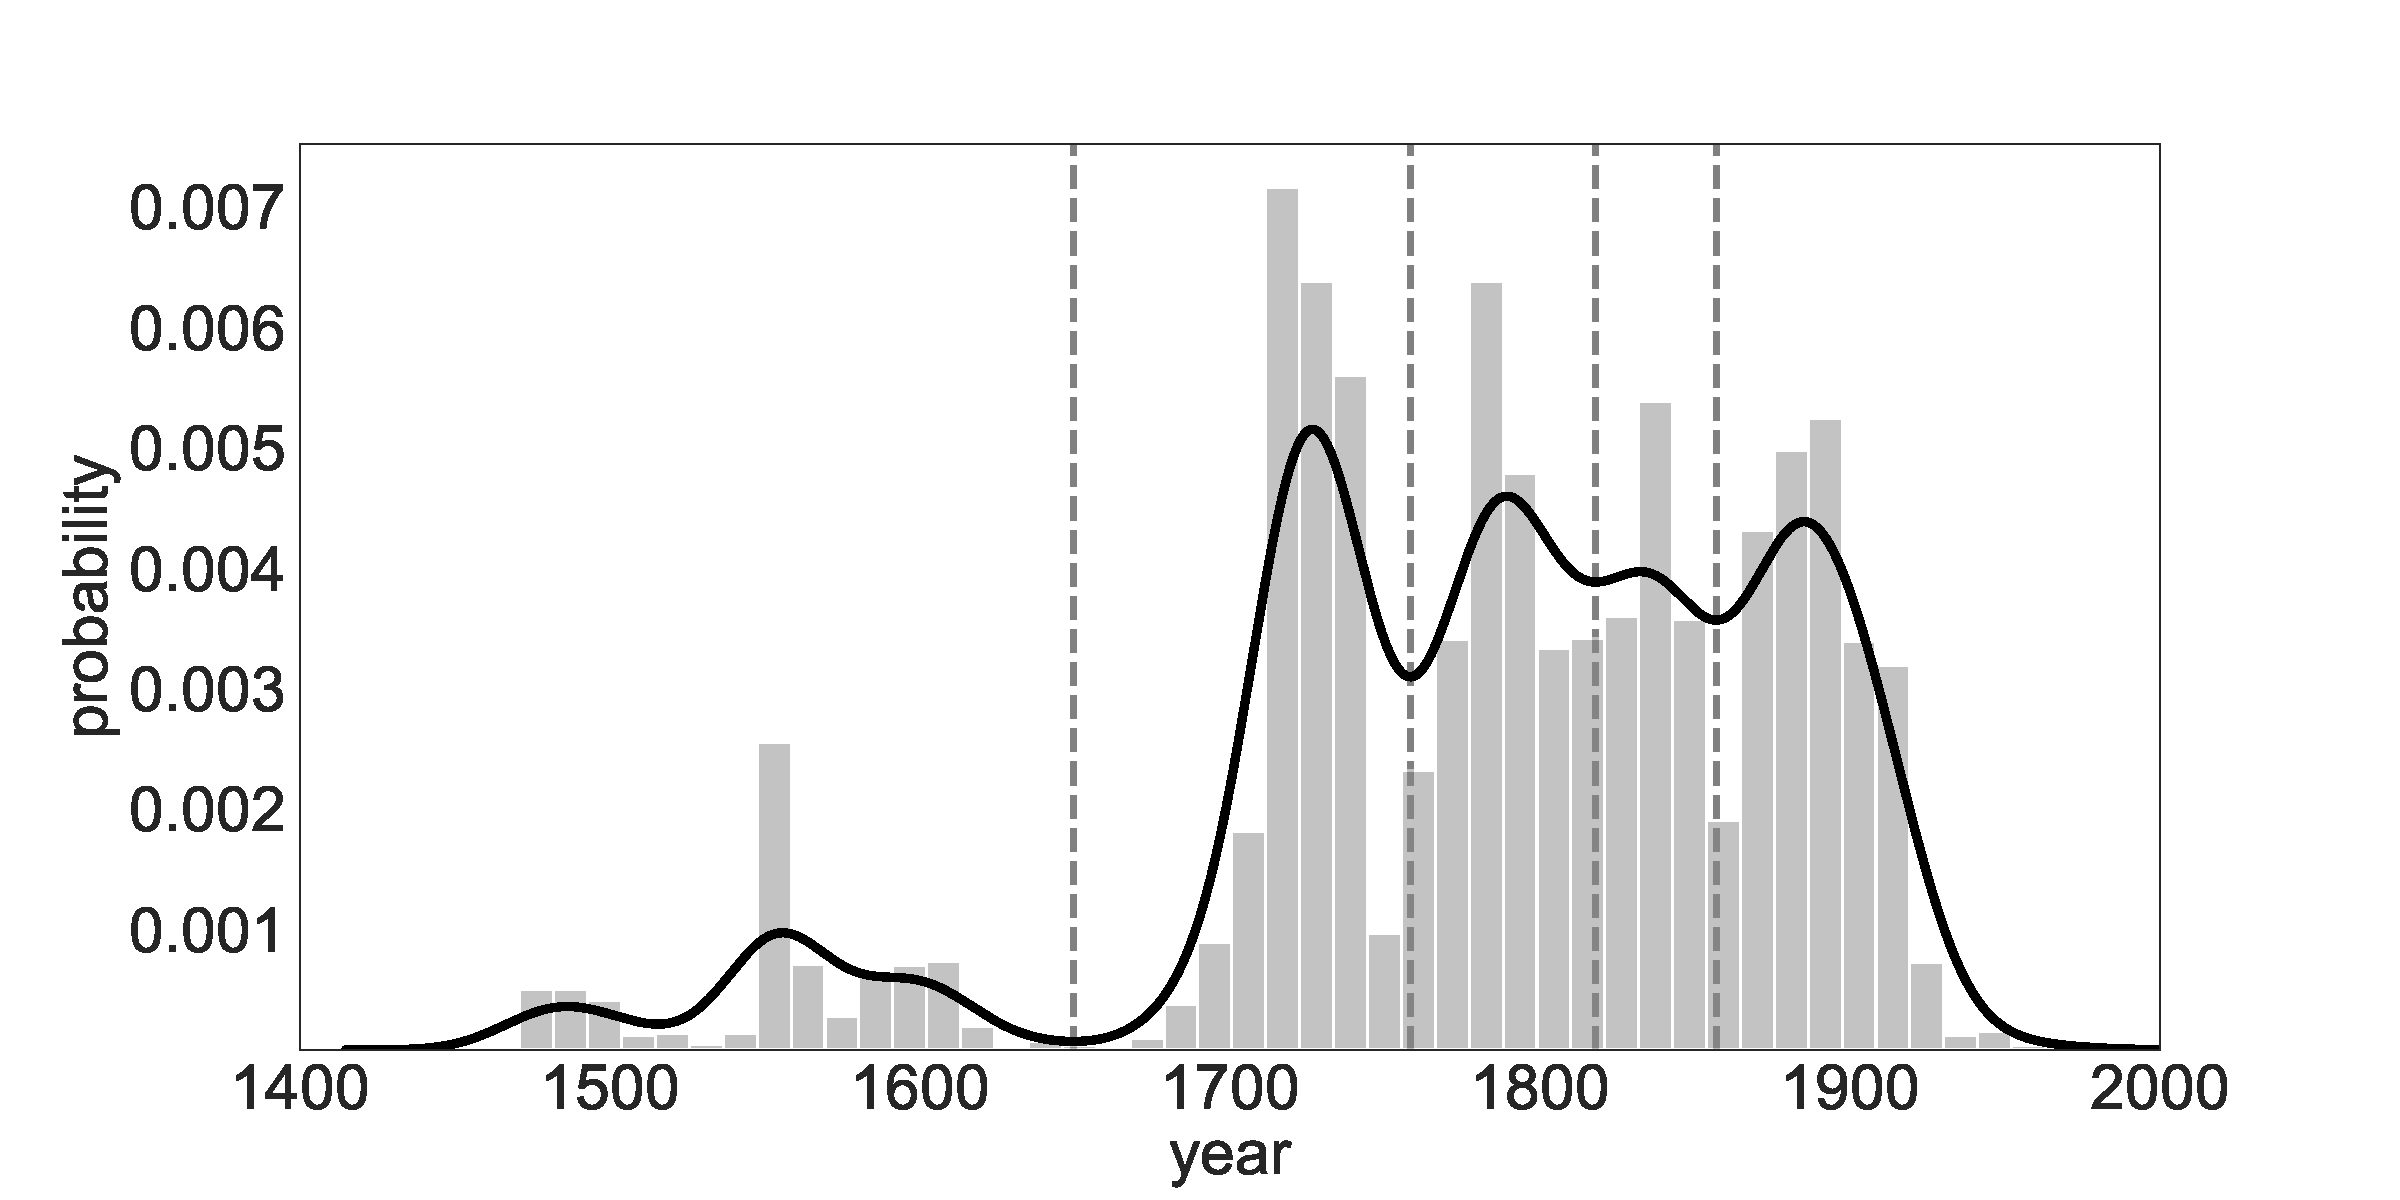
\includegraphics[width=\linewidth,height=.8\textheight,keepaspectratio]{img/Figure1.pdf}
        \caption{Historical distribution of pieces in the corpus.}
        \label{fig:piece_dist}
    \end{figure}
\end{frame}

\begin{frame}{Assumptions}
    \begin{enumerate}
        \item pieces can be represented by pitch-class counts
        \item enharmonic equivalence
        \item transpositional invariance
    \end{enumerate}

    \pause
    
    All of these assumptions are highly questionable, especially on a large historical scale!
    
    \pause
    
    $\Longrightarrow$ explitic modeling
\end{frame}

\begin{frame}{An example}
    \begin{figure}
        \centering
        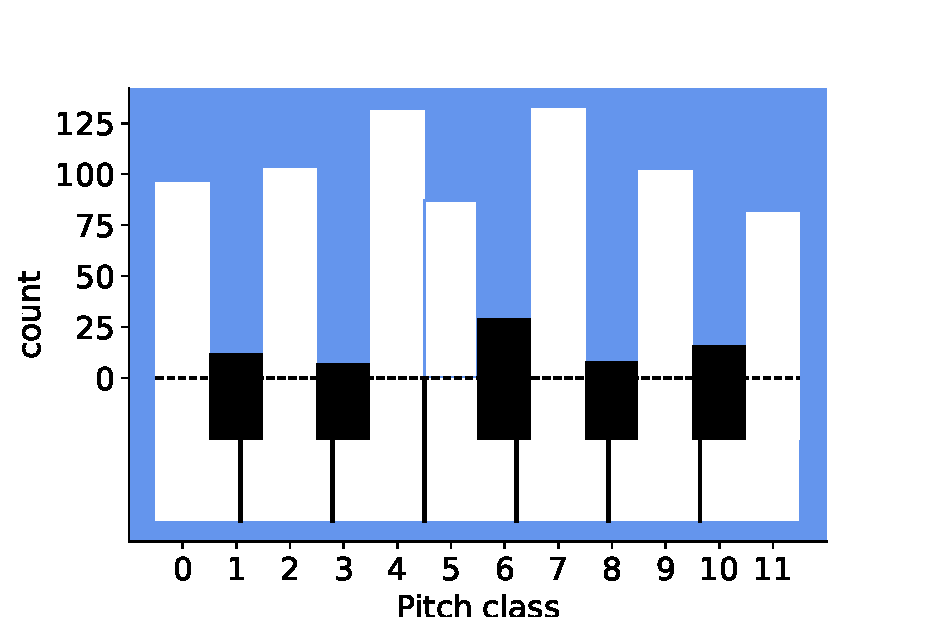
\includegraphics[width=.6\linewidth]{img/piano_pitch_class.eps}
        \caption{Pitch-class counts of an example piece in C~major.}
    \end{figure}
\end{frame}

\begin{frame}{The model}

    Abstand zwischen zwei Stücken $p$ und $q$ im \emph{key space} $\mathbb K$:
    \begin{equation}
        d_{\mathbb K} (p,q) = \left\| \frac{p}{\sum_i p_i} - \frac{q}{\sum_i q_i} \right\|_2,
    \end{equation}

    \pause

    Abstand zwischen zwei Stücken $p$ und $q$ im \emph{mode space} $\mathbb M$:
    \begin{equation}
        d_\mathbb M (p,q) =
        \min_{i\in\mathbb Z_{12}} d_{\mathbb K}(\sigma_i(p), q) = \min_{i\in\mathbb Z_{12}} d_{\mathbb K}(p, \sigma_{i}(q)),
    \end{equation}
\end{frame}

\begin{frame}{The model}

    The optimal mode:

    \begin{equation}\label{map_key}
        (R^*,M^*)= \operatorname*{argmax}_{(R,M)\,\in\,\mathbb Z_{12}\times\{1, \ldots, m\}} p(R,M\mid T,P,D).
    \end{equation}
    
    In words: Given a piece $P$ in a time period $T$ in the corpus $D$, the best (mode, root) pair $(M^*, R^*)$ is the one
    that maximizes the probabilty $p$.
\end{frame}

\begin{frame}{Automatically finding modes}
    \begin{figure}
        \centering
        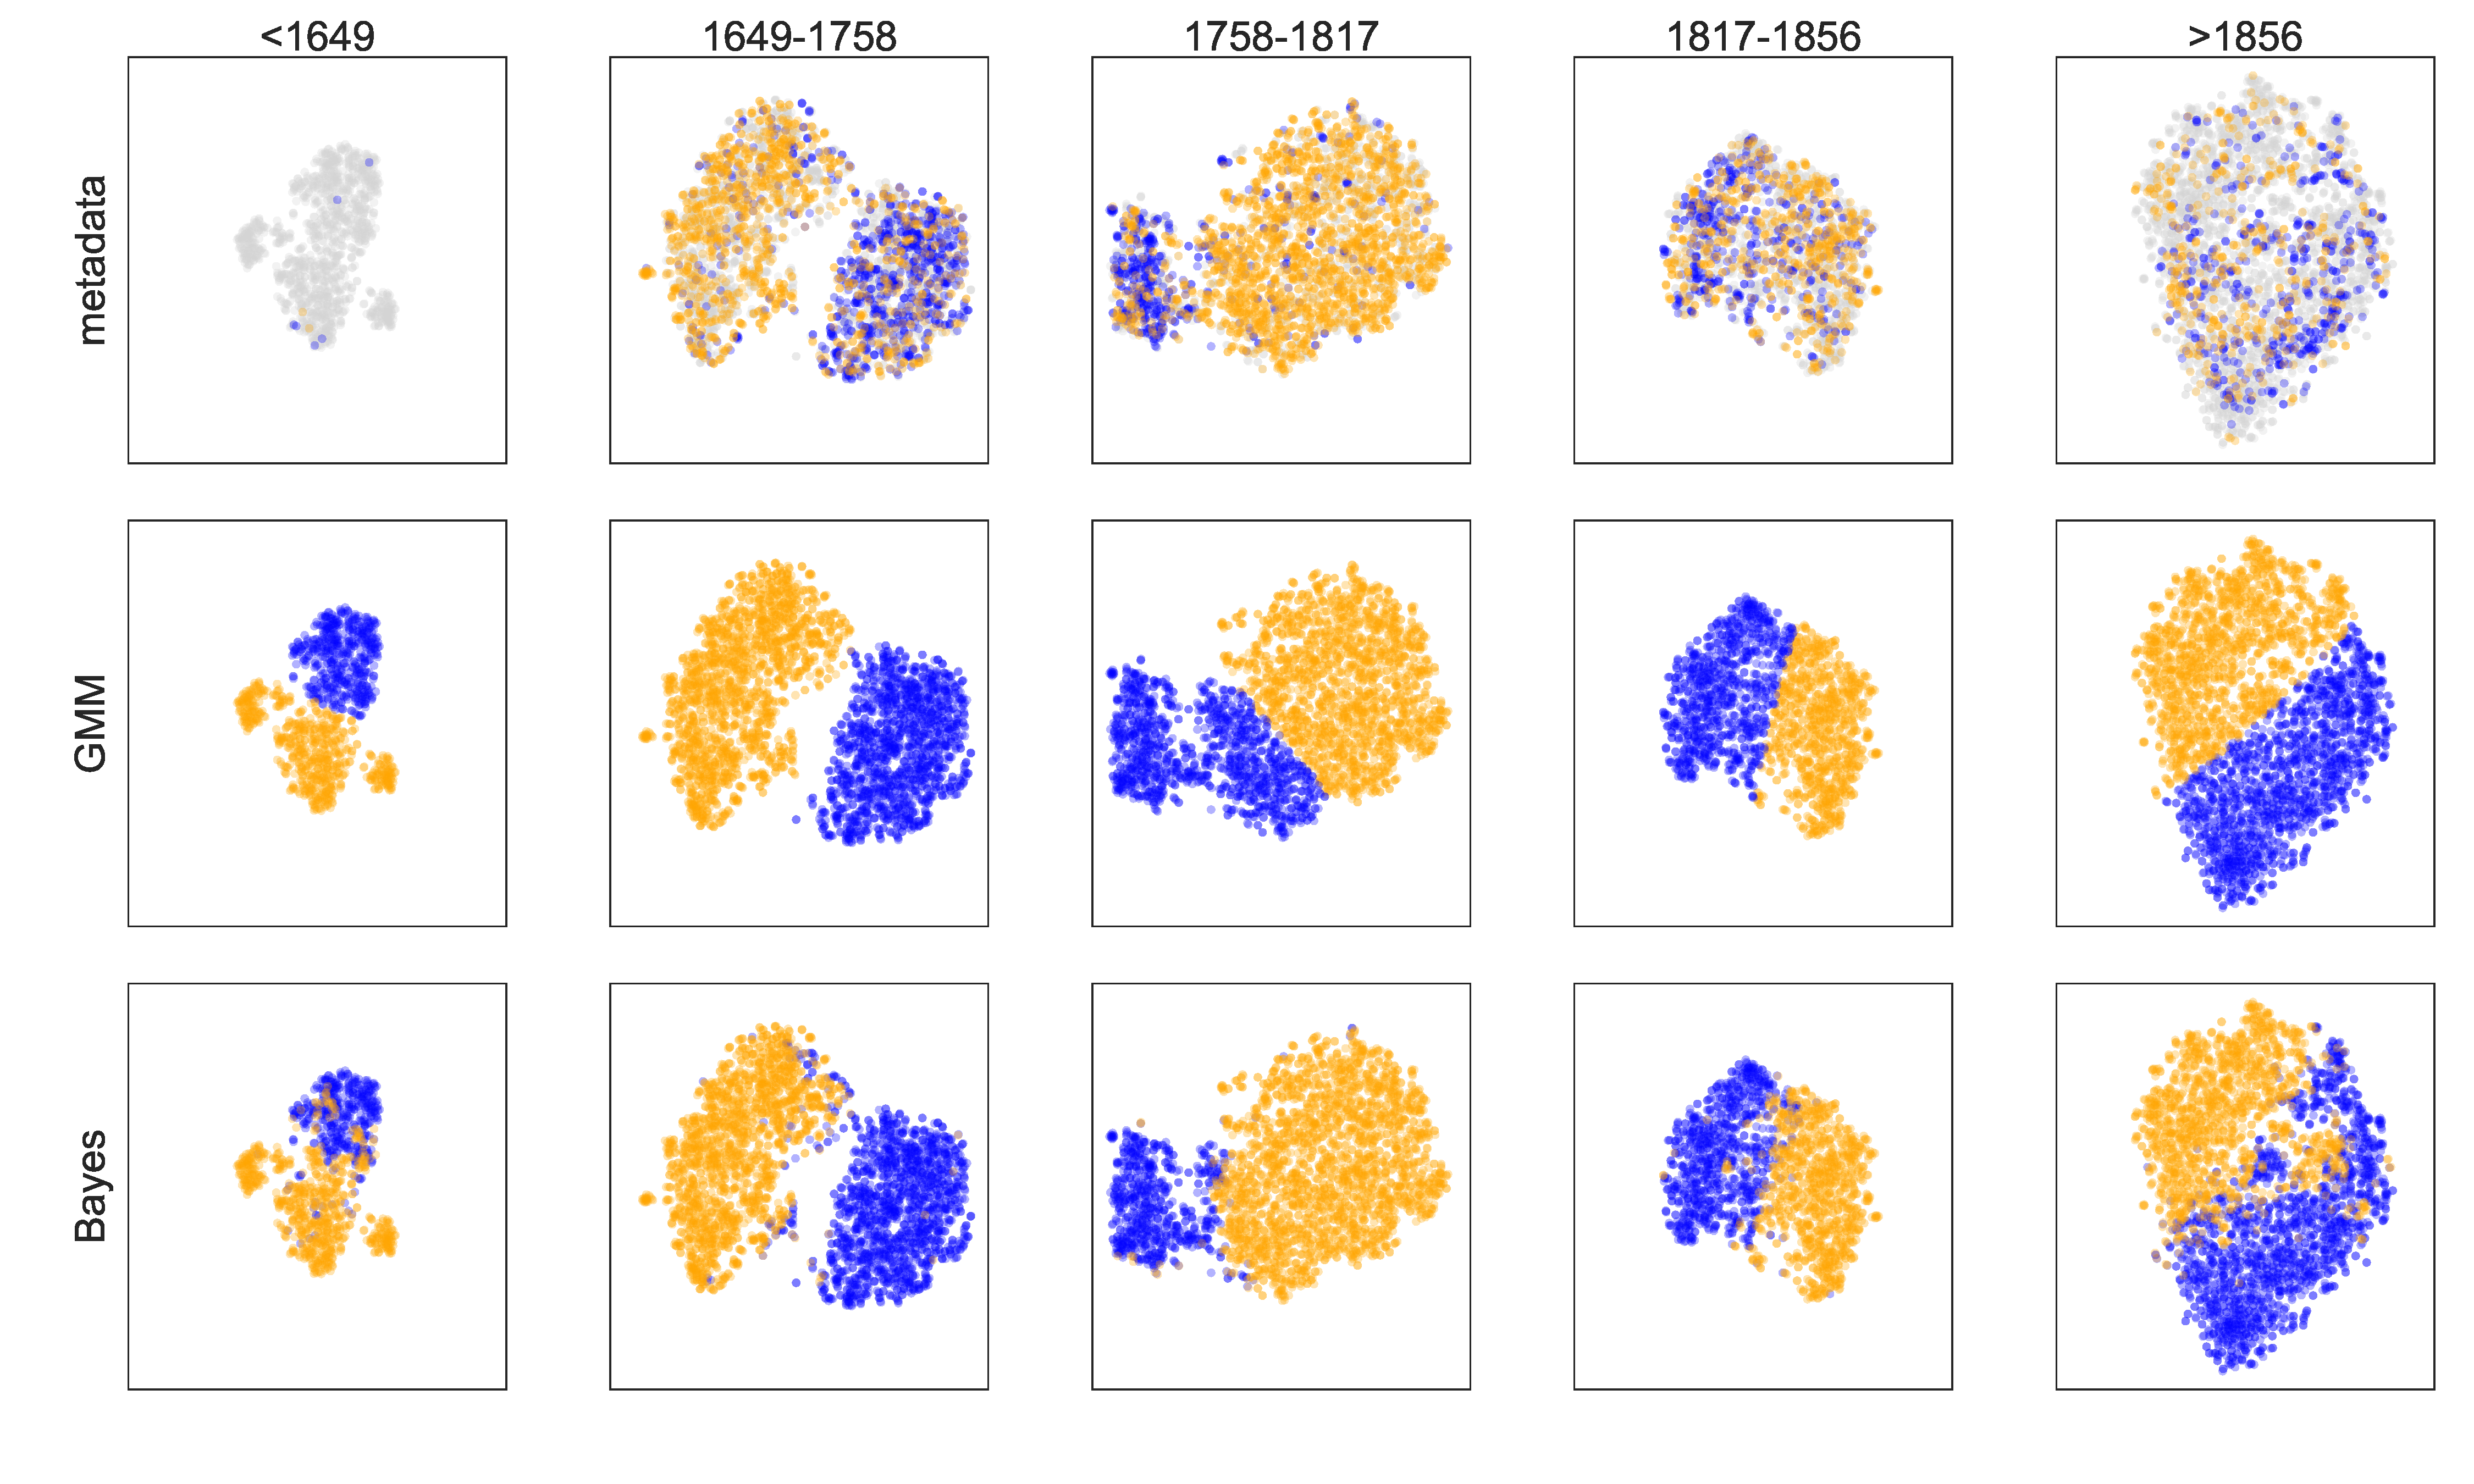
\includegraphics[width=\linewidth,height=.8\textheight,keepaspectratio]{img/Figure4.pdf}
        \caption{Three models for automatic mode finding.}
        % \label{fig:piece_dist}
    \end{figure}
\end{frame}

\begin{frame}{Quality of the model}
    \begin{figure}
        \centering
        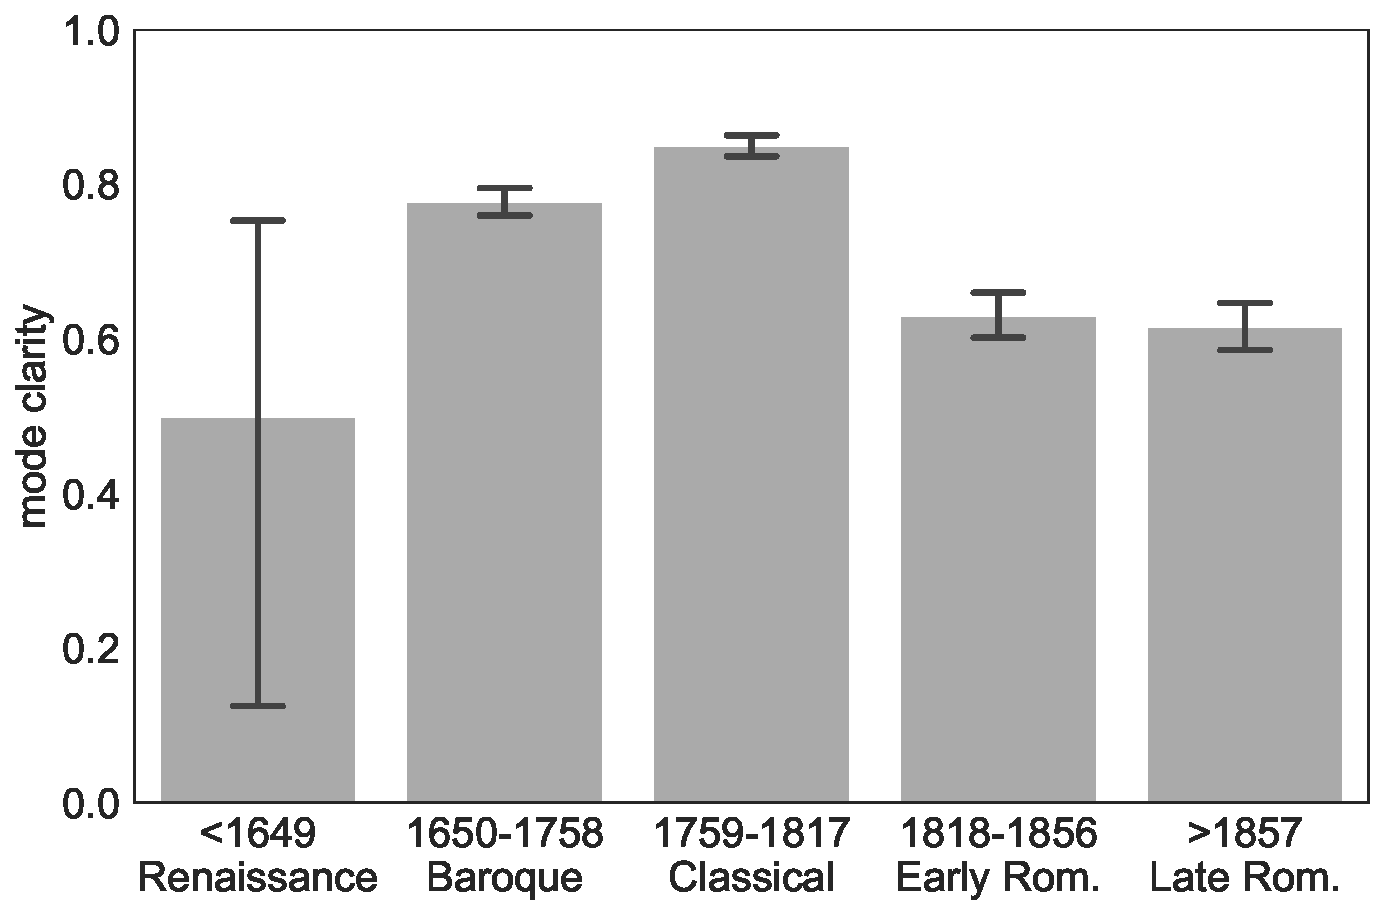
\includegraphics[width=\linewidth,height=.7\textheight,keepaspectratio]{img/Figure5.pdf}
        \caption{Accuracy scores of our model in five historical periods.}
        % \label{fig:piece_dist}
    \end{figure}
\end{frame}

\begin{frame}{The major and minor modes}

    Pitch-class distributions of all pieces in the Baroque and Classical periods:

    \begin{figure}
        \centering
        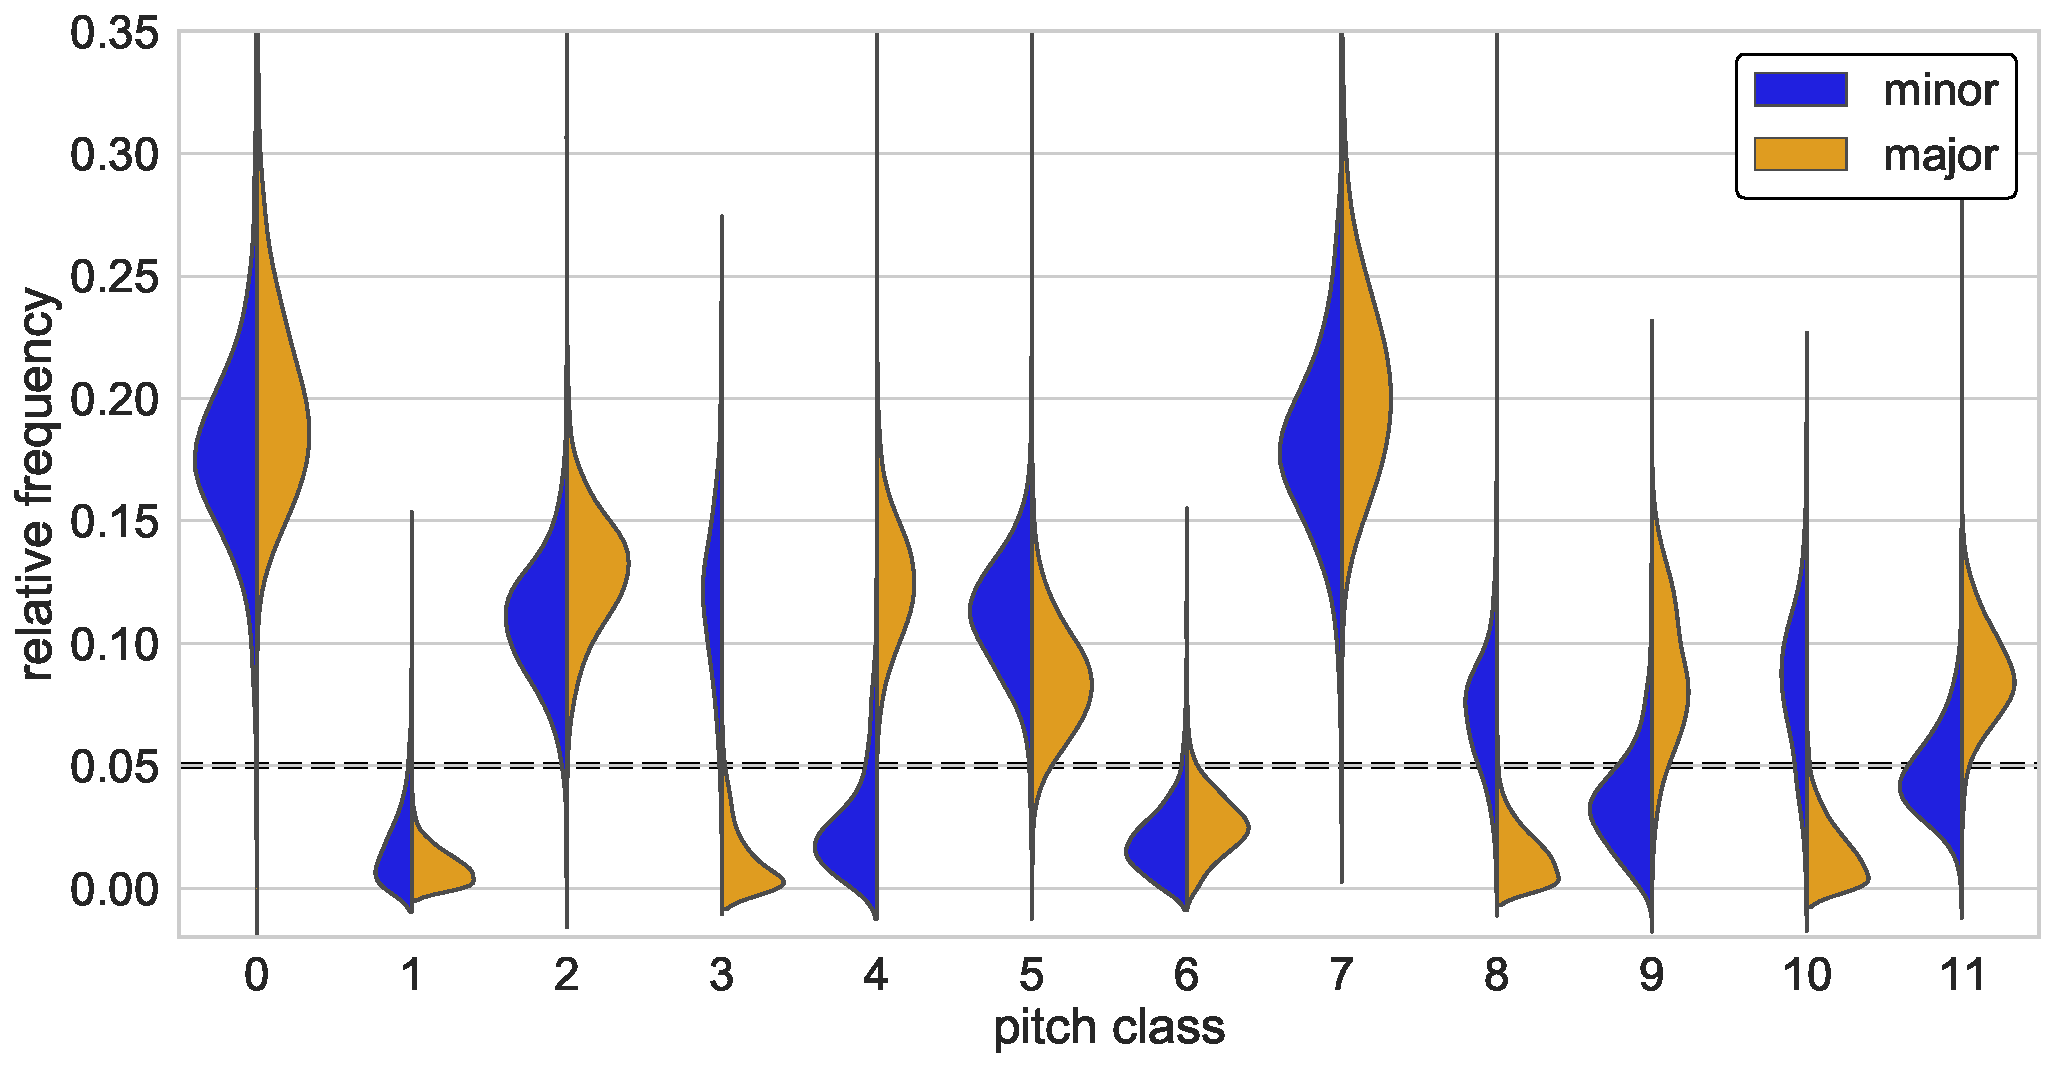
\includegraphics[width=\linewidth,height=.7\textheight,keepaspectratio]{img/Figure8.pdf}
        \caption{Pitch-class distribution of the major and minor modes.}
        % \label{fig:piece_dist}
    \end{figure}
\end{frame}

\begin{frame}{Modes in the Renaissance}
    \begin{figure}
        \centering
        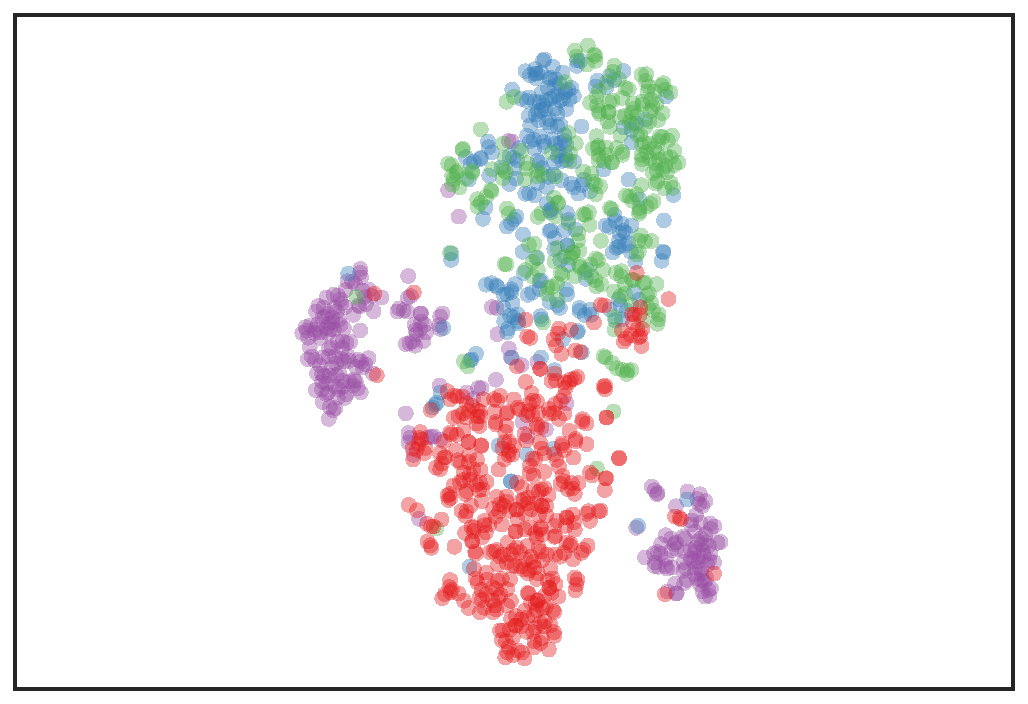
\includegraphics[width=\linewidth,height=.7\textheight,keepaspectratio]{img/Figure6.pdf}
        \caption{Clustering into four modes in the Renaissance.}
        % \label{fig:piece_dist}
    \end{figure}
\end{frame}

\begin{frame}{Modes in the Renaissance}
    \begin{figure}
        \centering
        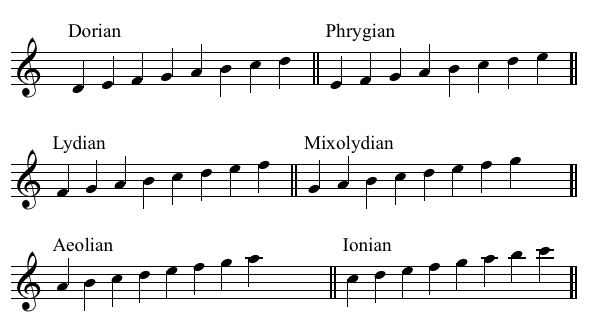
\includegraphics[width=.6\linewidth]{img/renaissance_modes.png}
        \caption{Six modes in early music.}
    \end{figure}
\end{frame}

\begin{frame}{Modes in the Renaissance}
    \begin{columns}
        \begin{column}{.6\linewidth}
            \begin{figure}
                \centering
                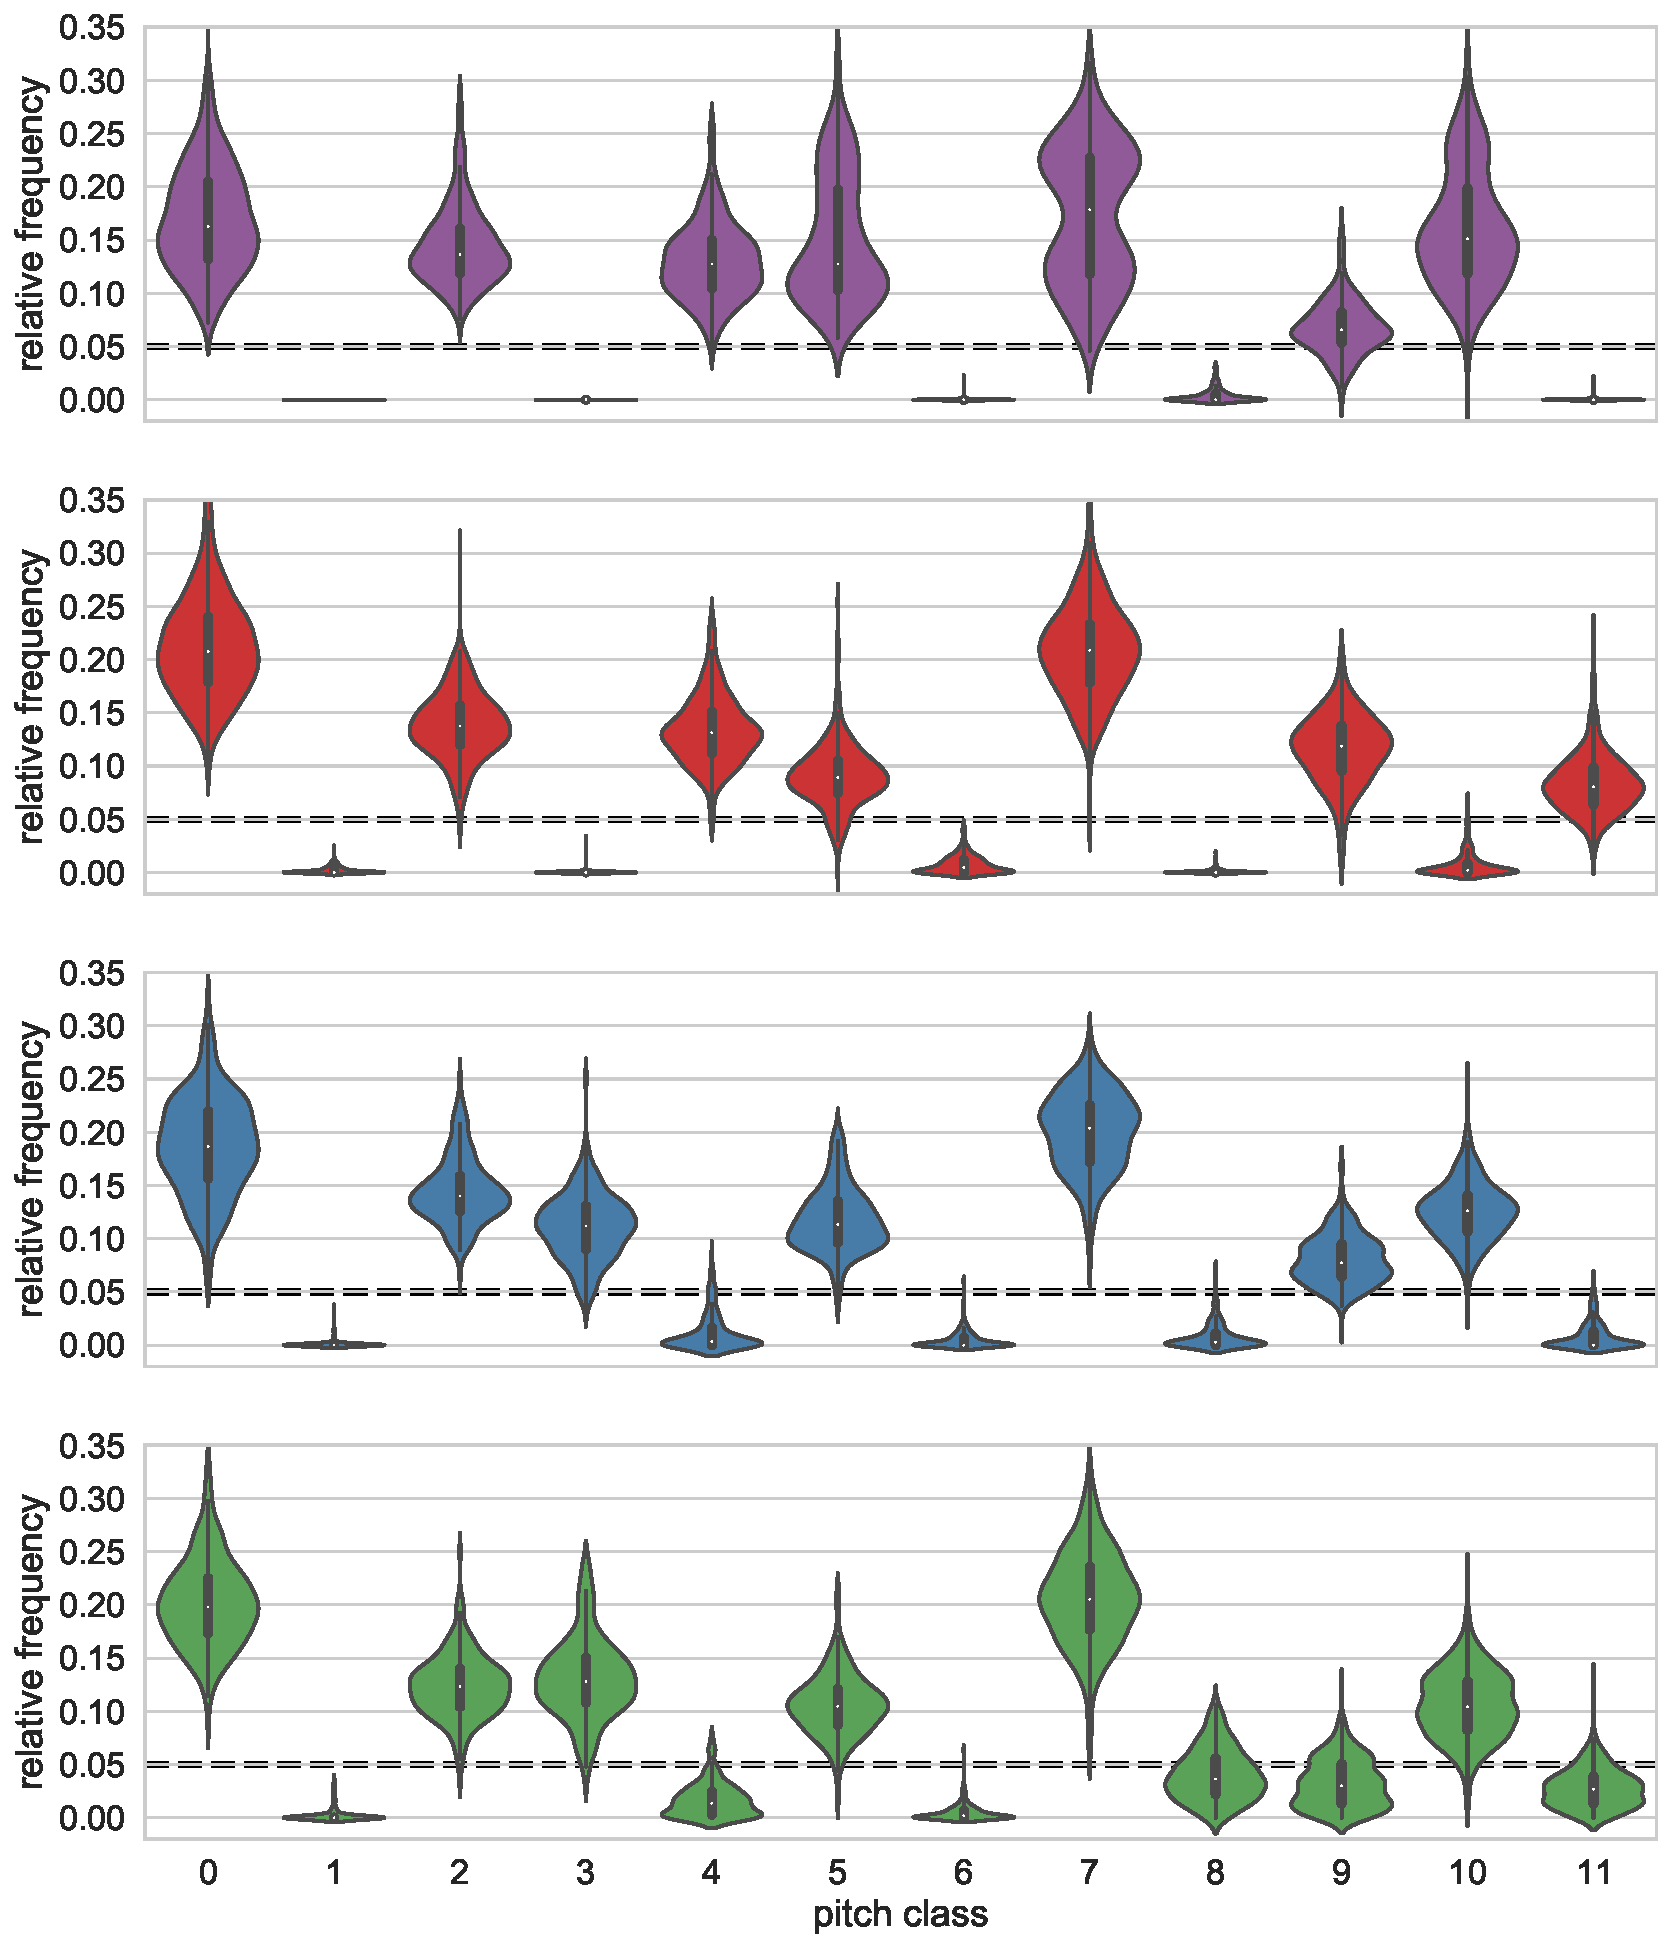
\includegraphics[width=\linewidth,height=.8\textheight,keepaspectratio]{img/Figure7.pdf}
                \caption{Pitch-class distribution of Renaissance modes.}
                % \label{fig:piece_dist}
            \end{figure}
        \end{column}
        \hfill
        \begin{column}{.4\linewidth}
            Four modes emerge in the Renaissance
            
            \begin{itemize}
                \item Mixolydian (violet)
                \item Ionian (red)
                \item Dorian (blue)
                \item Aeolian/Dorian (green)
            \end{itemize}
        \end{column}
    \end{columns}
\end{frame}

\begin{frame}{This course}
    \begin{itemize}
        \item The examples in this course are much simpler!
        \item Quality > Quantity
    \end{itemize}
\end{frame}